\everymath{\displaystyle}
\documentclass{beamer}
% \documentclass[handout]{beamer}

%\usepackage[pdftex]{color,graphicx}
\usepackage{amsmath,amssymb,amsfonts}

\mode<presentation>
{
  % \usetheme{Darmstadt}
  % \usetheme[hideothersubsections]{Hannover}
  % \usetheme[hideothersubsections]{Goettingen}
  \usetheme[hideothersubsections, right]{Berkeley}

  \usecolortheme{seahorse}
  % \usecolortheme{dolphin}
  \usecolortheme{rose}
  % \usecolortheme{orchid}

  \useinnertheme[shadow]{rounded}

  % \setbeamercovered{transparent}
  \setbeamercovered{invisible}
  % or whatever (possibly just delete it)
}

\mode<handout>{
  \setbeamercolor{background canvas}{bg=black!5}
  \usepackage{pgfpages}
  \pgfpagesuselayout{4 on 1}[a4paper,border shrink=5mm, landscape]
}

\usepackage[brazilian]{babel}
% or whatever

% \usepackage[latin1]{inputenc}
\usepackage[utf8]{inputenc}
% or whatever

\usepackage{times}
%\usepackage[T1]{fontenc}
% Or whatever. Note that the encoding and the font should match. If T1
% does not look nice, try deleting the line with the fontenc.


\title%[] % (optional, use only with long paper titles)
{Reprodutibilidade de estudos, e indicadores na Ciência}

\subtitle
{} % (optional)

\author%[] % (optional, use only with lots of authors)
{Felipe Figueiredo}% \and S.~Another\inst{2}}
% - Use the \inst{?} command only if the authors have different
%   affiliation.

\institute[INTO] % (optional, but mostly needed)
{Instituto Nacional de Traumatologia e Ortopedia
}
  % \inst{1}%
  % Department of Computer Science\\
  % University of Somewhere
  % \and
  % \inst{2}%
  % Department of Theoretical Philosophy\\
  % University of Elsewhere}
% - Use the \inst command only if there are several affiliations.
% - Keep it simple, no one is interested in your street address.

\date%[] % (optional)
{}

% \subject{Talks}
% This is only inserted into the PDF information catalog. Can be left
% out. 



% If you have a file called "university-logo-filename.xxx", where xxx
% is a graphic format that can be processed by latex or pdflatex,
% resp., then you can add a logo as follows:

\pgfdeclareimage[height=1.6cm]{university-logo}{../logo}
\logo{\pgfuseimage{university-logo}}



% Delete this, if you do not want the table of contents to pop up at
% the beginning of each subsection:
\AtBeginSubsection[]
%\AtBeginSection[]
{
  \begin{frame}<beamer>{Sumário}
    \tableofcontents[currentsection,currentsubsection]
  \end{frame}
}


% If you wish to uncover everything in a step-wise fashion, uncomment
% the following command: 

% \beamerdefaultoverlayspecification{<+->}


\begin{document}

\begin{frame}
  \titlepage
\end{frame}

\begin{frame}{Sumário}
  \tableofcontents
  % You might wish to add the option [pausesections]
\end{frame}


%% Template
% \section{}

% \subsection{}

% \begin{frame}{}
%   \begin{itemize}
%   \item 
%   \end{itemize}
% \end{frame}

% \begin{frame}
%   \begin{columns}
%     \begin{column}{5cm}
%     \end{column}
%     \begin{column}{5cm}
%     \end{column}
%   \end{columns}
% \end{frame}

% \begin{frame}{}
%   \includegraphics[height=0.4\textheight]{file1}
%   \includegraphics[height=0.4\textheight]{file2}
%   \includegraphics[height=0.4\textheight]{file3}
%   \begin{figure}
%     \caption{}
%   \end{figure}
% \end{frame}

% \begin{frame}{}
%   \begin{definition}
%   \end{definition}
%   \begin{example}
%   \end{example}
%   \begin{block}{Exercício}
%   \end{block}
% \end{frame}

\section{Apresentação}

\subsection{O docente e material online}

\begin{frame}{Docente}
  \begin{block}{Nome}
    Felipe Figueiredo
  \end{block}
  \begin{block}{Email}
    \url{prof.felipefigueiredo@gmail.com}

    \bigskip
    \small
    \alert{Atenção:} Salve-o como contato e use o endereço salvo, para mitigar a chance de {\bf estravio}!
    \footnote{O endereço felipefigueiredo@gmail.com {\bf não é meu}!}
  \end{block}
\end{frame}

\begin{frame}{Material online}
  Todo o material didático será disponibilizado na página da disciplina, que fica no Site abaixo
  \begin{block}{Site (http / https)}
    \small
    \url{sites.google.com/site/proffelipefigueiredo/}
  \end{block}
  % Adicionalmente, avisos importantes podem ser divulgados no blog
  % \begin{block}{Blog}
  %   \small
  %   \url{http://proffelipefigueiredo.blogspot.com.br/}
  % \end{block}

  \bigskip
  O endereço não é de fácil memorização, portanto uma busca no Google é o melhor caminho.

  \bigskip
  Você pode procurar pelo meu nome (Felipe Figueiredo)

  \bigskip
  \bigskip
  Porém...
\end{frame}

\begin{frame}{Google: felipe figueiredo}
  \begin{center}
    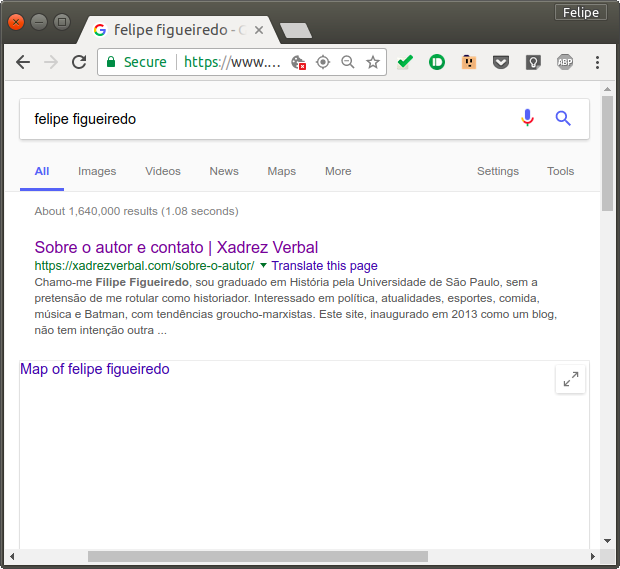
\includegraphics[height=.7\textheight]{Intro/felipefigueiredo-not1}
    \begin{exampleblock}{}
      \begin{center}
        {\bf Não sou Historiador}
      \end{center}
    \end{exampleblock}
  \end{center}
\end{frame}

\begin{frame}{Google: dr felipe figueiredo}
  \begin{center}
    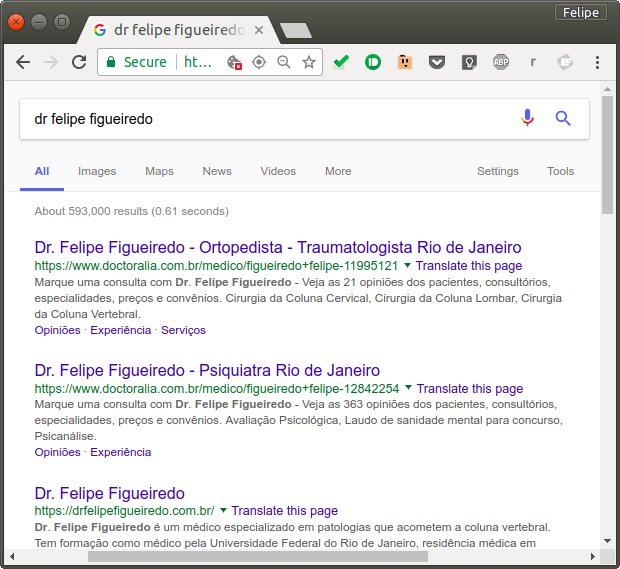
\includegraphics[height=.7\textheight]{Intro/felipefigueiredo-not2}
    \begin{exampleblock}{}
      \begin{center}
        {\bf Não sou Psiquatra ou Ortopedista}
      \end{center}
    \end{exampleblock}
  \end{center}
\end{frame}

\begin{frame}{Google: prof felipe figueiredo}
  \begin{center}
    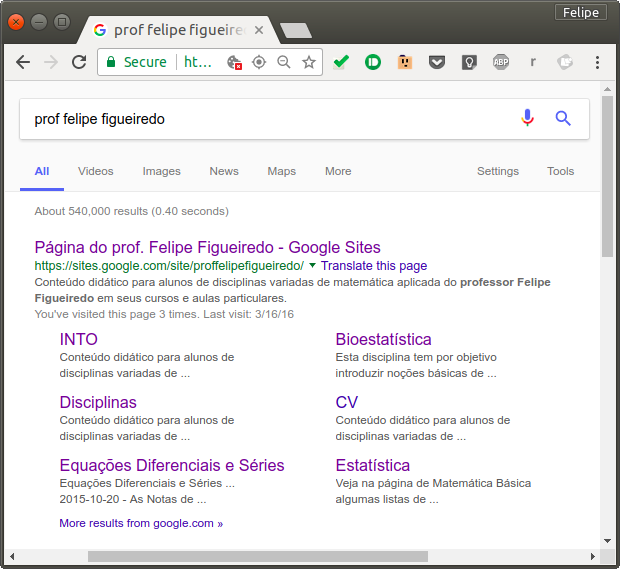
\includegraphics[height=.7\textheight]{Intro/felipefigueiredo}
    \begin{exampleblock}{}
      \begin{center}
        Este que vos fala, a seu dispor.
      \end{center}
    \end{exampleblock}
  \end{center}
\end{frame}

\begin{frame}{Material online}
  \begin{center}
    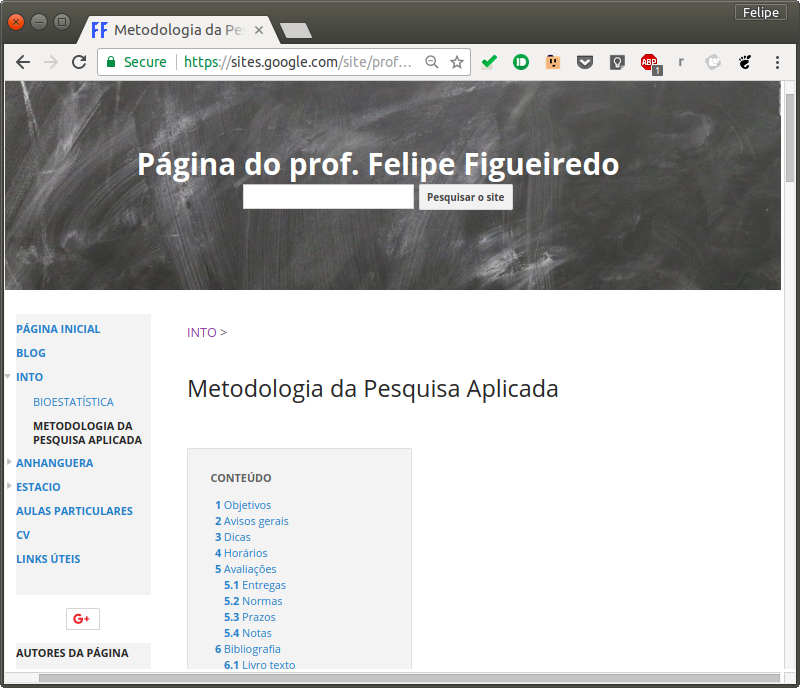
\includegraphics[height=.7\textheight]{Intro/pg-disciplina}
    \begin{exampleblock}{}
      \begin{center}
        PDFs das aulas, artigos, livros, vídeos, exercícios...
      \end{center}
    \end{exampleblock}
  \end{center}
\end{frame}

\subsection{A disciplina}

\begin{frame}[label=objetivo]{Objetivos de aprendizagem}

  \begin{block}{Principal}
    \begin{itemize}
    \item Redação de um projeto
    \end{itemize}
  \end{block}

  \begin{block}{Secundários}
    Oferecer uma introdução suave a
    \begin{itemize}
    \item Metodologia científica
    \item Redação científica
    \end{itemize}
  \end{block}

\end{frame}

\begin{frame}{Bibliografia}
  \begin{block}{Livro texto}
    {\bf Metodologia do Trabalho Científico: Métodos e Técnicas da Pesquisa e do Trabalho Acadêmico} (PRODANOV, Cleber Cristiano; de FREITAS, Ernani Cesar, 2013).
  \end{block}
  \begin{itemize}
  \item Outros materiais online linkados na página da disciplina.
  \end{itemize}
\end{frame}

\begin{frame}{O que esperar da disciplina}
  \tiny
  \begin{enumerate}
  \item<2,6> {Reprodutibilidade de estudos, e indicadores na Ciência (Hirsch,2005; Garfield, 2006)}
  \item<2,6> {Métodos científicos}
  \item<2,6> {Tópicos de escrita científica} (Gopen e Swan, 1990)
  \item<2,6> {Problema, Hipótese, variável}
  \item<2,6> {Tópicos em formulação de hipóteses}
  \item<2,6> \alert<6>{Etapas da Pesquisa (Planejamento e eventuais fracassos)}
  \item<3,6> {Estrutura do Projeto I - Conteúdo}
  \item<3,6> {Estrutura do Projeto II – Forma}
  \item<3,6> {Citações, Referências e Plágio}
  \item<4,6> {Revisão bibliográfica para a Introdução e Resumo}
  \item<4,6> {Tópicos de Busca Bibliográfica (Google-fu, {\em et al})}
  \item<5,6> \alert<6>{Tópicos em Estratégias de Apresentação}
  \item<1-> \alert<6>{Seminários individuais}
  \item<1-> \alert<6>{Seminários individuais}
  \item<1-> \alert<6>{Seminários individuais}
  \end{enumerate}
  \uncover<6>{ Os itens em vermelho indicam entregas de avaliação.}
\end{frame}

\begin{frame}{Avaliação}
  \begin{block}{Primeira entrega}
    Proposta inicial (sumário)
  \end{block}

  \pause

  \begin{block}{Segunda entrega}
    \begin{itemize}
    \item Projeto (padrão ABNT);
    \item Rascunho da apresentação da defesa.
    \end{itemize}
  \end{block}

  % \begin{itemize}
  % \item Escrita de um projeto {\em ad-hoc}.
  %       \end{itemize}
  % \item<3-> Seminário de defesa do projeto.
  % \end{itemize}
\end{frame}

\againframe{objetivo}

\begin{frame}{}
  \begin{block}{}
    {\bf Não subestime a dificuldade da escrita!}

    Acredite, escrever é muito difícil.
  \end{block}

  \bigskip
  \bigskip
  \uncover<2>{E pra provar...}
\end{frame}

\subsection{Exercício}

\begin{frame}{Exercício}
Escreva um procedimento detalhado para pregar um prego em um sabão

  \begin{center}
    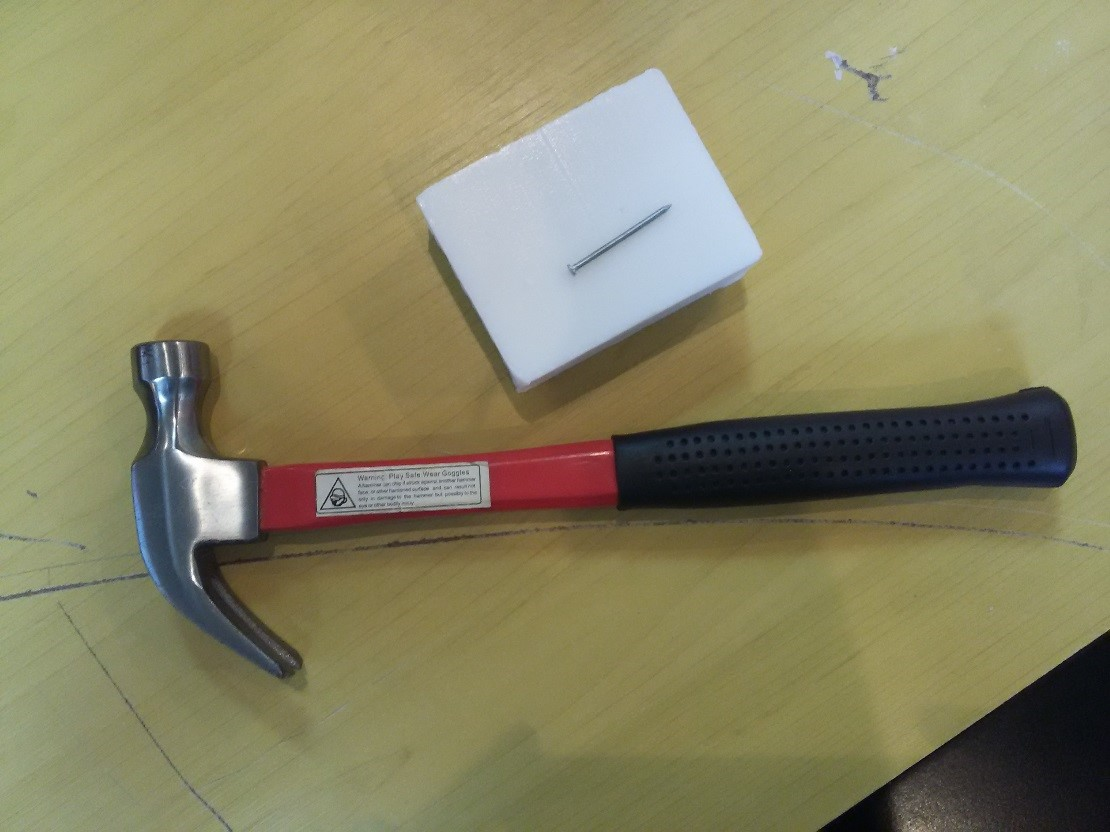
\includegraphics[width=0.8\textwidth]{Intro/pregomartelo}
  \end{center}
\end{frame}

\section{Ciência e Cientometria}

\subsection{Conceitos preliminares}

% \subsection{Verdade}

\begin{frame}{Verdade}
  \begin{columns}
    \begin{column}{6cm}<1-> ``{\em When you have eliminated the
        impossible, whatever remains, however improbable, must be the
        truth.}'' Sherlock Holmes
    \end{column}
    \begin{column}{4cm}<1->
      
\includegraphics[height=0.4\textheight]{Intro/truth}
    \end{column}
  \end{columns}
\end{frame}

% \subsection{Evidências}

% \subsection{Dados, Informação e Conhecimento}

\begin{frame}{Dados, Informação e Conhecimento}
  \begin{center}
    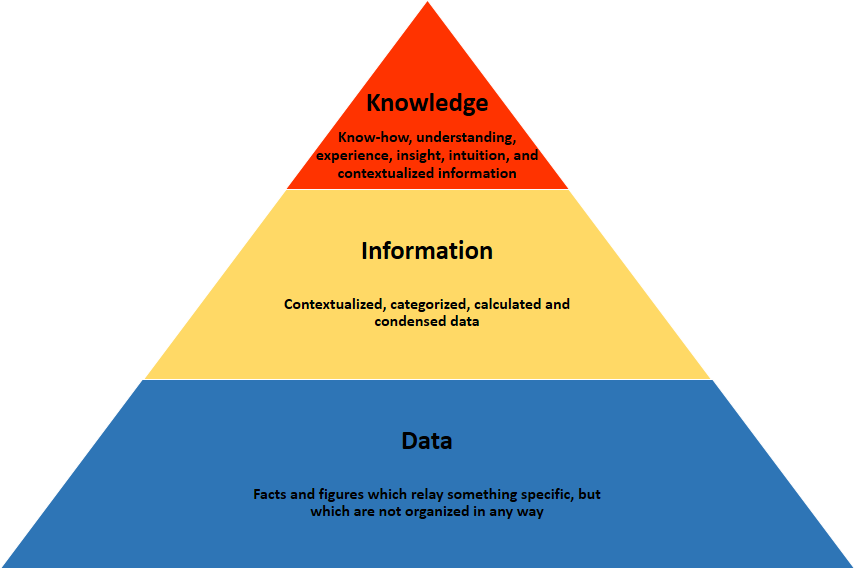
\includegraphics[height=0.9\textheight]{Intro/Knowledge_pyramid}
  \end{center}
  % \begin{figure}
  %   \caption{}
  % \end{figure}
\end{frame}

\begin{frame}{Dados, Informação e Conhecimento}
  % \item ``Evidence-based medicine (EBM) is the process of
  %   systematically reviewing, appraising and using clinical research
  %   findings to aid the delivery of optimum clinical care to
  %   patients''
    \begin{block}{Dados}
      elementos, códigos ou símbolos quantificáveis que são
    coletados em um experimento.
    \end{block}
    \begin{block}{Informação}
      agregação e interpretação de dados
    \end{block}
    \begin{block}{Conhecimento}
      agregação de um corpo de informações que tem significado e
      aplicabilidade prática
    \end{block}
\end{frame}


% \begin{frame}{Dados, Informação e Conhecimento}
%   \begin{example}
%     Dados do mercado financeiro: preço das ações da Petrobrás hoje
%   \end{example}
% \end{frame}

% \subsection{Tipos de conhecimento}

% \begin{frame}{Conhecimento Filosófico}
%   \begin{itemize}
%   \item Valorativo (parte de hipóteses que não podem ser observadas)
%   \item Racional (enunciados logicamente correlacionados)
%   \item Sistemático
%   \item Não verificável (conclusões não podem ser confirmadas nem
%     refutadas)
%   \item Infalível e exato (razão pura)
%   \end{itemize}
% \end{frame}

% \begin{frame}{Conhecimento Teológico}
%   \begin{itemize}
%   \item Valorativo
%   \item Inspiracional
%   \item Sistemático
%   \item Não verificável
%   \item Infalível e exato (divino)
%   \end{itemize}
% \end{frame}

% \begin{frame}{Conhecimento Popular}
%   \begin{itemize}
%   \item Valorativo (estados de ânimo e emoções)
%   \item Reflexivo (não pode ser generalizado)
%   \item Assistemático
%   \item Verificável (no cotidiano)
%   \item Falível e inexato (percepções do dia a dia)
%   \end{itemize}
% \end{frame}

\begin{frame}{Conhecimento Científico}
  \begin{itemize}
  \item Factual
  \item Contingente (\alert{experimento} ao invés de razão pura)
  \item Sistemático 
  \item \alert{Verificável}
  \item Falível (não é definitivo)
  \item Aproximadamente exato (novos dados podem derrubar teorias
    anteriores)
  \end{itemize}
\end{frame}

% \begin{frame}{Classificação da Ciência}
%   \begin{center}
%     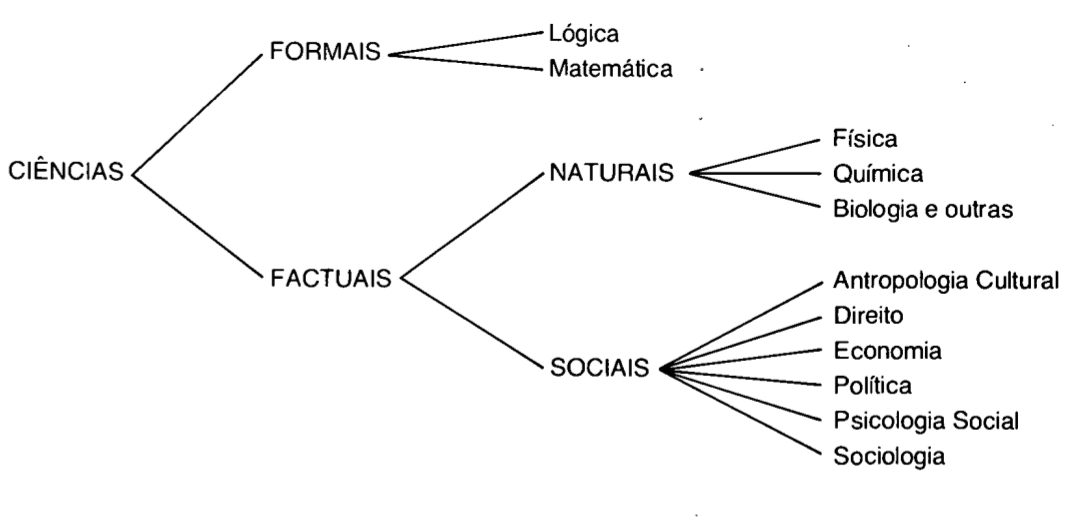
\includegraphics[width=\textwidth]{Intro/ciencias}
%   \end{center}
% \end{frame}

% \subsection{Resumo}

% \begin{frame}{Conhecimento Científico x Senso Comum}
%   \begin{itemize}
%   \item Um mesmo objeto ou fenômeno \alert{pode} ser observado por
%     qualquer tipo de conhecimento
%   \item diferença: forma de observação
%   \item Ciência
%     \begin{itemize}
%     \item reprodutível
%     \item acúmulo incremental
%     \item autoavaliação ou correção
%     \end{itemize}
%   \end{itemize}
% \end{frame}

\begin{frame}{Conhecimento Científico x Senso Comum}
  \begin{columns}
    \begin{column}{5cm}
      \begin{center}
        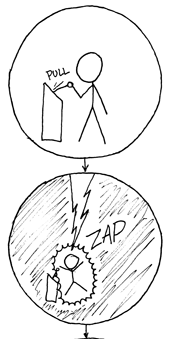
\includegraphics[width=0.55\textwidth]{Intro/the_difference1}
      \end{center}
    \end{column}
    \begin{column}{5cm}
      \begin{center}
        \begin{center}
          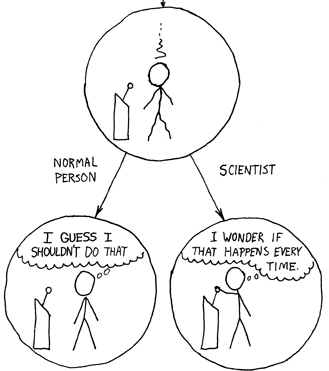
\includegraphics[width=\textwidth]{Intro/the_difference2}
        \end{center}
      \end{center}
    \end{column}
  \end{columns}

https://xkcd.com/242/
\end{frame}

\subsection{Indicadores de Pesquisadores}

\begin{frame}{Pense...}
  \begin{center}
    Qual é a diferença entre um cientista famoso\ldots

    \bigskip
    \ldots e um desconhecido?
  \end{center}
\end{frame}

\begin{frame}{Para quê indicadores de pesquisadores?}
  \begin{itemize}
  \item Agraciados com o prêmio Nobel: se destacam por impacto indiscutível
  \item E os outros mortais? Como aferir o impacto da produção de um cientista?
  \item Como comparar a relevância entre dois cientistas?
  \end{itemize}
\end{frame}

\subsubsection{Algumas propostas}

\begin{frame}{Como {\em medir} a ``relevância'' de um pesquisador?}
  \begin{itemize}
  \item Como atribuir uma métrica objetiva à produção de um cientista?
  \item Como detectar trabalhos {\em revolucionários}?
  \item Como fazer tudo isso, respeitando nossa intuição (e.g. Newton, Einstein, Darwin, \ldots)?
  \end{itemize}
\end{frame}

\begin{frame}{Algumas propostas}
  \begin{itemize}
  \item Número de artigos publicados (total, ou por ano)
  \item Total de citações recebidas
  \item Número de citações por artigo
  \end{itemize}
\end{frame}

\begin{frame}{Número de artigos}
  \begin{block}{Premissa}
    Quanto maior a produtividade, maior a relevância do cientista.
  \end{block}
  \begin{itemize}
  \item ``Pastel chinês''
  \item Alguns autores produzem MUITOS artigos, incluindo muitos de qualidade
  \item Estes são exceção, não a regra
  \item Em geral, muitos artigos não implicam em muito conhecimento ou informação gerados
  \item A publicação só tem impacto, se é lida e usada como base para novos trabalhos (i.e.: \alert{citada})
  \end{itemize}
\end{frame}

\begin{frame}{Total de citações recebidas}
  \begin{block}{Premissa}
    Quanto mais citações recebidas, maior a relevância da produção para a comunidade.
  \end{block}
  \begin{itemize}
  \item Trabalhos muito citados inflacionam esta métrica
  \item Um pesquisador pode ter apenas um trabalho muito citado, e vários menos relevantes
  \item Pesquisadores mais antigos acumulam citações há mais tempo que os jovens
  \end{itemize}
\end{frame}

\begin{frame}{Total de citações por artigo}
  \begin{block}{Premissa}
    Média alta de citações por artigo indica uma produtividade média relevante
  \end{block}
  \begin{itemize}
  \item A média é ``melhor'' que o total, simplifica a análise (sumariza)
  \item Permite comparar cientistas de ``idades'' diferentes
  \item Publicar muitos artigos, aumenta a dificuldade de manter uma média alta!
  \item Trabalhos muito citados também podem inflacionar a média (perda de relevância)
  \end{itemize}
\end{frame}

\begin{frame}{Vantagens x desvantagens}
  Total de artigos
  \begin{block}{Vantagens}
    Mede produtividade do pesquisador
  \end{block}
  \begin{block}{Desvantagens}
    Não mede importância ou impacto dos artigos
  \end{block}

\vfill
Fonte: Hirsch, 2005.
\end{frame}

\begin{frame}{Vantagens x desvantagens}
Total de citações
  \begin{block}{Vantagens}
    Mede o impacto total do pesquisador
  \end{block}
  \begin{block}{Desvantagens}
    Difícil de determinar, e pode ser inflacionado por poucos trabalhos bem sucedidos
  \end{block}

\vfill
Fonte: Hirsch, 2005.
\end{frame}

\begin{frame}{Vantagens x desvantagens}
Citações por artigo
  \begin{block}{Vantagens}
    Permite comparar pesquisadores de idades diferentes
  \end{block}
  \begin{block}{Desvantagens}
    Difícil de determinar, premia pouca produtividade, penaliza grande produtividade
  \end{block}

\vfill
Fonte: Hirsch, 2005.
\end{frame}

\subsubsection{Índice H}

\begin{frame}{O Índice H}
  \begin{definition}
    Um pesquisador tem índice $h$ se ele é coautor de $h$ artigos com \alert{pelo menos} $h$ citações.
  \end{definition}
  \begin{example}[Top $h$ entre os físicos]
    E. Witten tem índice $h=110$.

    Então ele tem 110 artigos com pelo menos 110 citações cada.

    \uncover<3>{(monstro)}
  \end{example}

\vfill
Fonte: Hirsch, 2005.
\end{frame}

\begin{frame}{Vantagens}
  \begin{itemize}
  \item Fácil de calcular (basta ordenar os artigos por número de citação)
  \item Não possui as desvantagens dos critérios anteriores
  \item Mede o impacto geral da produção do pesquisador
  \item Dá uma ``ideia'' do número total de citações
  \item BR: o CV Lattes incorpora a opção de calcular e exibir seu índice $h$
  \end{itemize}

\vfill
Fonte: Hirsch, 2005.
\end{frame}

\begin{frame}{Outros físicos/astrônomos}
  \begin{itemize}
  \item<1-> A.J. Heeger: $h=107$
  \item<1-> M.L. Cohen e A.C. Gossard: $h=94$
  \item<1-> P.W. Anderson: $h=91$
  \item<1-> \ldots
  \item<1-> S.W. Hawking: $h=61$
  \item<2-> $h$ médio dos aceitos na National Academy of Sciences em 2005: $h=44$
  \end{itemize}

\vfill
Fonte: Hirsch, 2005.
\end{frame}

\begin{frame}{Prêmio Nobel de Física}
  \begin{itemize}
  \item $h$ médio entre os agraciados com o prêmio Nobel nos últimos 20 anos: $h=41$
  \item $84\%$ destes tem $h$ maior ou igual a 30
  \end{itemize}

\vfill
Fonte: Hirsch, 2005.
\end{frame}

\begin{frame}{E na área biológica/biomédica?}
  \begin{itemize}
  \item População: cientistas mais citados no período 1983--2002
  \item<1-> S.H. Snyder: $h=191$
  \item<1-> D. Bailtimore: $h=160$
  \item<1-> R.C. Gallo: $h=154$
  \item<1-> \ldots
  \item<1-> A. Ulrich: $h=120$
  \item<2-> $h$ médio dos 36 aceitos na National Academy of Sciences em 2005: $h=57$
  \end{itemize}

\vfill
Fonte: Hirsch, 2005.
\end{frame}

\begin{frame}{Observações}
  \begin{itemize}
  \item O perfil do índice $h$ visivelmente varia para cada área do conhecimento
  \item Com o tempo, o acúmulo de citações aumenta o $h$ do pesquisador
  \item O índice $h$ permite comparar o impacto de dois pesquisadores da mesma área.
  \end{itemize}

\vfill
Fonte: Hirsch, 2005.
\end{frame}

% \subsubsection{Índice M}

% \begin{frame}{Uma desvantagem do índice H}
%   \begin{itemize}
%   \item Com o tempo, o acúmulo de citações aumenta o índice $h$ do pesquisador
%   \item Isso favorece pesquisadores mais antigos
%   \item Pesquisadores jovens podem ter um impacto grande, que não será detectado pelo índice $h$
%   \item Conclusão: o tempo faz com que não seja possível comparar o impacto pesquisadores com ``idades'' muito diferentes
%   \end{itemize}
% \end{frame}

% \begin{frame}{O Índice M}
%   \begin{definition}
%     \begin{displaymath}
%       m \approx \frac{h}{n}
%     \end{displaymath}
%   \end{definition}
%   \begin{block}{Significado}
%     Normalizar o índice $h$ em relação ao tempo total de produção ($n$ anos de publicações)
%   \end{block}

% \vfill
% Fonte: Hirsch, 2005.
% \end{frame}

% \begin{frame}{Interpretação}
%   \begin{itemize}
%   \item Manter $h=10$ por 10 anos: $m=1$
%   \item Manter $h=10$ por 5 anos: $m=2$
%   \item Manter $h=10$ por 20 anos: $m=0.5$
%   \end{itemize}
% \end{frame}

% \begin{frame}{Exemplos Físicos/Astrônomos}
%   \begin{itemize}
%   \item<1-> A.J. Heeger: $m=2.38$
%   \item<1-> M.L. Cohen e A.C. Gossard: $m=2.04$ e $m=2.09$
%   \item<1-> P.W. Anderson: $m=1.88$
%   \item<1-> \ldots
%   \item<1-> S.W. Hawking: $m=1.59$
%   \item<2-> $m$ médio prêmio Nobel: $m=1.14$
%   \item<3-> Obs: Agraciados com o prêmio Nobel tipicamente têm $m$ menor que pesquisadores ativos ($49\%$ da amostra tem $m<1$)
%   \end{itemize}

% \vfill
% Fonte: Hirsch, 2005.
% \end{frame}

% \begin{frame}{Observações}
%   \begin{itemize}
%   \item O índice $m$ mede o impacto da produção, sem ser distorcido pelo tempo de carreira
%   \item Um índice $m\approx 1$ indica um grande impacto
%   \item Um índice $m\approx 2$ indica um impacto excepcional
%   \item Um índice $m\approx 3$ indica criaturas únicas
%   \end{itemize}

% \vfill
% Fonte: Hirsch, 2005.
% \end{frame}

\subsection{Indicadores de Revistas}

\subsubsection{Relevância}

\begin{frame}
  \begin{itemize}
  \item Como vimos, o número de citações é um fator importante na determinação do impacto de uma obra
  \item Aumentar a visibilidade da publicação: maior chance de citações
  \item Revistas mais lidas oferecem essa maior chance
  \item Mas também são mais exigentes no peer-review
  \end{itemize}
\end{frame}

\subsubsection{Qualis da CAPES}

\begin{frame}{Qualis da CAPES}
  \begin{itemize}
  \item Lista de revistas categorizadas por ``qualidade''
  \item Níveis: A1, A2, B1 -- B5, C
  \item Considera áreas individualmente: uma revista pode ser A1 em uma área, e A2 em outra
  \item Implicitamente, leva em conta o Fator de Impacto (?)
  \item Publicações em revistas indexadas pelo Qualis são contabilizadas para pontuação da CAPES
  \end{itemize}
\end{frame}

\subsubsection{Fator de Impacto}

\begin{frame}{Objetivos, usos e abusos}
  \begin{itemize}
  \item Fator de Impacto: Journal Impact Factor (JIF)
  \item Idealizado para medir a influência das citações de uma revista na literatura
  \item Tem sido utilizado para atribuir valor acadêmico aos trabalhos publicados na revista
  \item Também: aferir a qualidade de indivíduos, instituições e departamentos
  \end{itemize}

  \vfill
  Fonte: McVeigh, Mann (2009)
\end{frame}

\begin{frame}{O Journal Citation Report (JCR)}
  \begin{itemize}
  \item Relatório anual da Thomson Reuters (antiga Thomson ISI)
  \item Coleta todas as citações do Web of Science
  \item Classificado por áreas do conhecimento
  \end{itemize}
\end{frame}

\begin{frame}{O Journal Impact Factor (JIF)}
  \begin{definition}
    JIF é a razão entre as citações recebidas e o número de artigos citáveis
  \end{definition}
  \begin{itemize}
  \item Revistas novas não têm fator de impacto
  \item o JIF é atualizado anualmente
  \item O número de citações é obtido do relatório anual JCR
  \item BR: Incorporado no CV Lattes
  \end{itemize}
\end{frame}

\begin{frame}{Número de citações}

  \begin{itemize}
  \item Artigos publicados nos 2 anos anteriores
  \item Citações recebidas pelos artigos
  \end{itemize}
  \begin{example}[para calcular o JIF de 2009]
    Citações em 2009 de artigos publicados entre 2007 e 2008
  \end{example}

  \vfill
  Fonte: Garfield (2006)
\end{frame}

\begin{frame}{Número de artigos citáveis}
São considerados citáveis principalmente:
  \begin{itemize}
  \item Artigos de pesquisa
  \item Reviews
  \end{itemize}
  \begin{block}{Desconsiderados}
    Cartas, editoriais, notícias, entrevistas, obituários, homenagens, \ldots
  \end{block}

  \vfill
  Fonte: Garfield (2006)
\end{frame}

\begin{frame}{Exemplo}
  \begin{example}[Fator de Impacto de 2009]
    \begin{displaymath}
      JIF = \frac{\text{citações em 2009 de publicações de 2007 + 2008}}{\text{publicações citáveis de 2007 + 2008}}
    \end{displaymath}
  \end{example}
  \begin{block}{Interpretação}
    Se uma revista tem $JIF=3$ em 2009, então suas publicações de 2007 e 2008 receberam na média 3 citações em 2009
  \end{block}
\end{frame}

\begin{frame}{Observações}
  \begin{itemize}
  \item O JIF não é perfeito: autocitações, ``cartéis'', etc
  \item Uma métrica objetiva é melhor que nenhuma métrica objetiva

  \end{itemize}
  \begin{block}{Parafraseando Hoeffel (1998) apud Garfield (2006)}
A experiência mostra que em cada área, as melhores revistas são aquelas em que é mais difícil ter sua publicação aceita, e estas revistas tem fator de impacto mais alto. (\ldots) O uso do IF como medida de qualidade é usual pois se encaixa na nossa opinião sobre quais são as melhores revistas de nossa área.
  \end{block}
\end{frame}

\section{Referências}

\begin{frame}{Referências}
  \begin{enumerate}
  \item<1-> HIRSCH, J.E. (2005) An index to quantify an individual's scientific research output, PNAS.
  \item<1-> GARFIELD, E. (2006) The History and Meaning of the Journal Impact Factor, JAMA.
  \item<1-> McVEIGH, M.E.; MANN, S.J. (2009) The Journal Impact Factor Denominator, JAMA.
%  \item<1-> HUBBARD, S. C.; McVEIGH, M. E. (2011). Casting a wide net: The Journal Impact Factor numerator, Learned Publishing
%  \item<1-> HIRSCH, J.E. (2007) Does the h index have predictive power?, PNAS.
  \end{enumerate}
\end{frame}

\end{document}
